\chapter{Étude du nœud A}
Dans cette partie, nous étudierons un premier bloc du réseau. Nous calculerons les courbes d'arrivé du noeud et la courbe de service pour comprendre sa courbe de sortie et ainsi mesuré sa porter sur le reste du réseau.

Les tracés de l'ensemble des courbes a été obtenu par l'interpréteur en ligne \emph{http://realtimeatwork.com/minplus-playground}, il s'agit d'un interpréteur qui permet entre autre le tracé de courbes affines mais aussi le calcul en algèbre (min,+). 

Nous avons décidé de d'utiliser et de fixer les unités sur lesquelles nous baserons nos courbes. Nous avons choisi de travailler en \textbf{octets} (axe des ordonnées) et le temps (axe des abscisse) sera en \textbf{millisecondes}. Nous verrons en synthèse à ce rapport si nos choix pour ces unités étaient judicieux. \label{fixUnity}

\section{Courbes d'arrivée $\alpha$} 
Pour déterminer la courbe d'arrivée, nous allons tout d'abord analyser les données que nous pouvons receuillir sur le bloc A. Nous relevons deux flux d'entrée $v1$ et $v2$. Pour connaitre la courbe d'arrivée $\alpha^A$, nous devons tracer les deux courbes d'entrée des deux flux entrants, courbes que nous affichons en figure (\ref{fig:CA_1_2})

\begin{figure}[!ht]\label{fig:CA_1_2}
\centering
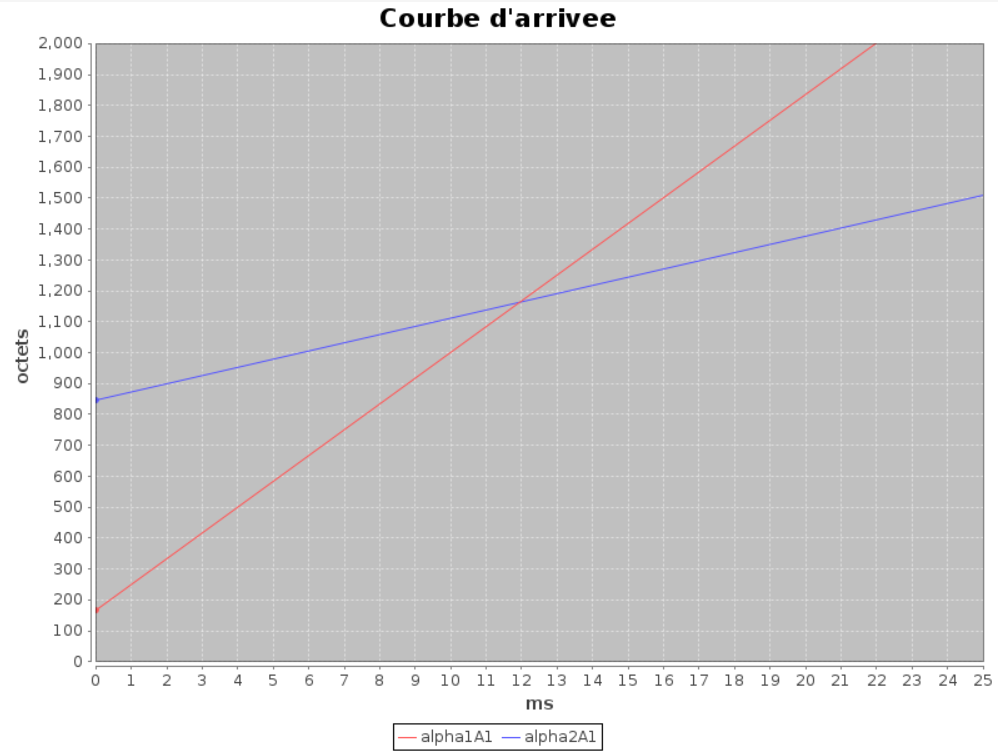
\includegraphics[width = .5\textwidth]{./I/images/alpha_1_2.png}
\caption{Courbe d'arrivée $\alpha$ du flux $v1$ (rouge) et du flux $v_2$ (bleu)}
\end{figure} 

Ces courbes ont été obtenu à l'aide des informations sur les $BAG$ et les $s_{max}$ de $v1$ et $v2$. Pour obtenir des données correspondantes aux unités choisis en \ref{fixUnity}, nous devons utiliser la relation suivantes qui lie la taille maximale d'une trame $L_j^{max}$ et la charge utile maximale $s_j^{max}$ d'un \emph{Virtual Link}(VL) $j$ :
\begin{align}\label{eqn:maxTrame}
L_j^{max} = max(s_j^{max},17)+47
\end{align}
Nous observons donc avec cette équation que la taille maximale d'une trame est strictement supérieure à $50$. A l'aide de cette équation, nous sommes capable d'établir la pente $a_j$ de la courbe des données maximales ainsi que son offset $b_j$ de décalage qui peuvent arrivées dans $A$ avec \begin{align}\label{eqn:penteOffset}
 &a_j = \frac{L_j^{max}}{BAG_j}\\
 &b_j = L_j^{max}
\end{align}

Dans notre cas, nous obtenons l'application numérique suivante : 
\begin{align*}
&a_1 = \frac{L_1^{max}}{BAG_1} = \frac{ max(s_j^{max},17)+47}{BAG_1} = \frac{167}{2} = 83.5\\
&b_1 =  max(s_j^{max},17)+47 = 167
\end{align*}
Avec l'interpréteur, nous pouvons obtenir la courbe affine avec la commande : \begin{verbatim}
alpha1A1 := affine(83.5, 167) //echelle octets/ms
\end{verbatim}

De même pour le flux $v2$,nous obtenons comme application numérique : \begin{align*}
&a_2 = 26.46\\
&b_2 = 847
\end{align*}
La courbe obtenu est de la forme sceau percé, nous avons une quantité maximale émise instantanément par le bloc $A$ et un débit moyen maximal.
\section{Courbe de service $\beta$}
Nous allons maintenant établir la courbe de service disponible par le nœud A. Cette fonction du port desortie de $A$ est établit en fonction de la latence technologique $\mu$ déterminé et du débit du port de sortie. Notre étude est calibré selon lesuniés défini en\ref{fixUnity}, il est donc important de respecter ces conditions dès maintenant pour éviter tout problème fuur d'unité. Nous relevons :\begin{align}\label{eqn:portSortie}
debit &= 100Mb/s = 12500\ Octets/ms\\
\mu &= 16\mu s = 0.016 ms
\end{align}

Pour établir cette fonction sur \emph{Network Calculus}, nous avons choisi d'établir une fonction affine qui admet comme pente le débit du port de sortie mais qui subit un décalage, i.e un \emph{delay} dans l'interpréteur, pour modéliser la latence technologique. La courbe en \ref{fig:serviceA} est obtenu avec la ligne de commande :
\begin{verbatim}
betaA := affine(12500,0) * delay(0.016) 
\end{verbatim}
\begin{figure}[!ht]\label{fig:serviceA}
\centering
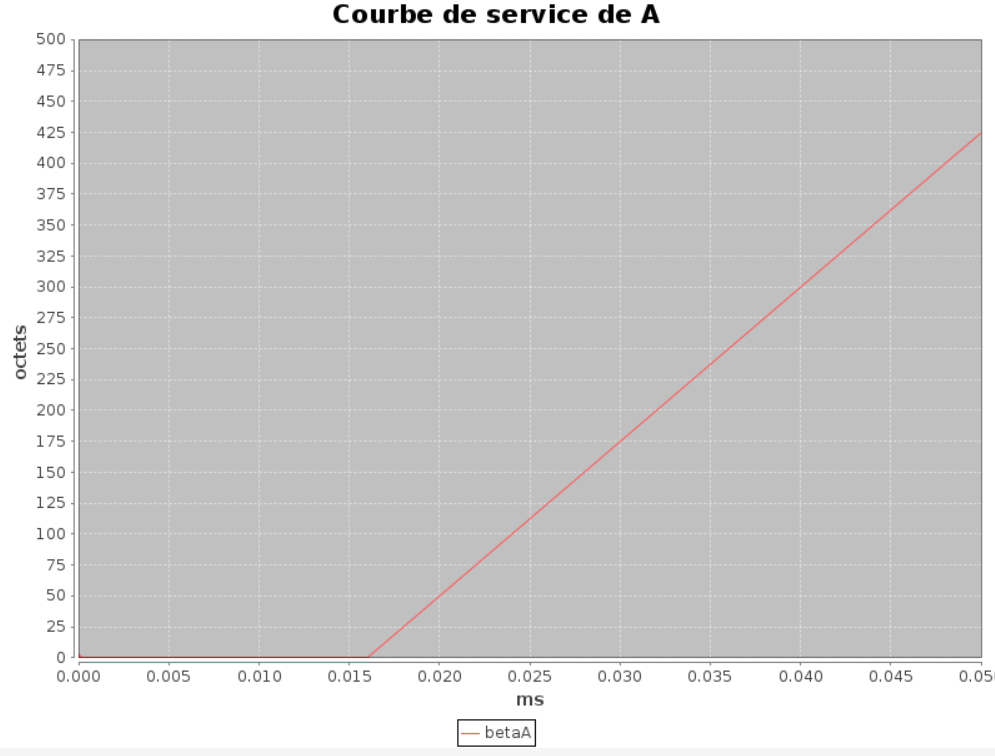
\includegraphics[width = .5\textwidth]{./I/images/beta_A.png}
\caption{Courbe de service du nœud A}
\end{figure} 

Cette courbe est du type latence-taux, car notre modèle admet une latence technologique et dispose d'un débit de sortie. Pour résumé, le modèle du nœud $A$ reçoit des données dans une courbe d'arrivé de type seau percé pour les traiter avec une courbe de service du type latence-tau. Selon nos estimations, le nœud va donc lisser le débit des flux $v1$ et $v2$.

\section{Courbe d'arrivé du nœud A}
Nous nous intéressons maintenant au cumul des flux dans l'entrée du nœud $A$.